\documentclass[a4paper,11pt]{report}
\usepackage[T1]{fontenc}
\usepackage[utf8]{inputenc}
\usepackage{lmodern}
\usepackage[francais]{babel}
\usepackage{graphicx}
\usepackage{setspace}
\usepackage{float}

\title{MonsterShip\texttrademark }
\author{Olivier \bsc{Boissard}, Kevin \bsc{Boulala},\\
Maxime \bsc{Dubois}, Antoine \bsc{Lavier}}
\date{Dernières modifications : \today}

\begin{document}

\maketitle
\setcounter{tocdepth}{1}
\tableofcontents

\chapter{Introduction}

    Le but de ce cahier des charges est de préciser les fonctionnalités du jeu
    MonsterShip. Le but de ce jeu est de contrôler un vaisseau, et de le rendre
    plus puissant que les vaisseaux des autres joueurs. Pour cela, le joueur pourra
    améliorer son vaisseau, en augmentant sa taille, et la puissance des armes
    et des boucliers, ou il pourra également attaquer les autres joueurs, afin
    d’endommager leurs vaisseaux. La seule ressource du jeu sera des monstres
    servant à la fois d’équipage pour le vaisseau, et de ressource de construction.
    En effet, ces monstres seront capables de fusionner avec le vaisseau, pour en
    améliorer les différentes capacités.

\chapter{Contexte}
      Le jeu MonsterShip sera développé sous forme d’application Java, et
    fonctionnera sur le portail web JBoss, à l’aide de Java Beans. La base de
    donnée sera sur un serveur MySQL. L’objectif est de créer un jeu qui puisse
    être vendu à tous les joueurs appréciant les jeux par navigateur. Pour cela,
    il doit être à la fois simple d’utilisation, pour que les joueurs occasionnels ne
    soient pas découragés dès le début, et suffisemment complet pour permettre
    aux joueurs de haut niveau de pouvoir mettre en place des stratégies qui
    leur permettraient d’avoir le vaisseau le plus puissant du jeu.

\chapter{Les objectifs}
    \section{Description générale du projet}
    C'est un jeu multijoueur par navigateur.\\

    Dans ce jeu le joueur contrôle et gère un vaisseau, le but étant de le faire grossir et prospérer.\\

    Pour se déplacer ou faire une action (attaquer, récolter des monstres), on utilise un système de points d'action qui se rechargent tous les jours.\\

    L’équipage du vaisseau est composé de petits monstres capables aussi bien de piloter le vaisseau en lui même, que de gérer les moteurs, utiliser les armes embarquées, etc. Pour faire prospérer son vaisseau, il faut utiliser son équipage comme une ressource de construction. Par exemple, le joueur souhaite avoir une arme plus puissante, le coût pour améliorer l’arme c’est de fusionner 2 membres de l’équipage avec cette arme. De même, le joueur peut fusionner des membres d'équipage avec le vaisseau, afin de l'agrandir pour pouvoir placer plus d'équipements (réacteurs, armes...).\\

    Pour améliorer son vaisseau, il faut explorer des planètes pour «récolter» d’autres monstres. Lors du recrutement, le joueur aura le choix entre une action instantannée lui donnant accès à un certain nombre de monstres contre des points d'action, ou une action plus longue qui lui permet d'obtenir des monstres en fonction du temps resté à la surface. Dans ce dernier cas, le joueur est sujet aux attaques et il est par la même occasion plus vulnérable, mais il ne consomme aucun point d'action. Il faudra trouver le bon équilibre entre faire grossir son vaisseau pour pouvoir ajouter des équipements et augmenter la puissance de ces équipements, mais en gardant un équipage suffisamment important pour que chaque fonctionnalité du vaisseau puisse être exploitée à son plein potentiel.\\

    Les joueurs peuvent se rencontrer et organiser des batailles purement statistiques. Le vainqueur repartirait avec potentiellement quelques dégâts mineurs, mais surtout avec de nouveaux membres d’équipages. Le perdant, lui repartira avec un vaisseau endommagé, ayant perdu une partie de ses capacités, et un équipage réduit.\\

    \section{Les enjeux}
    L'objectif est de créer un jeu capable de concurrencer OGame.\\

    Pour cela, le jeu vise une clientèle large, allant des joueurs occasionnels, qui ne se connectent quelques fois par semaine, voire par mois, aux joueurs hardcore capables de passer plusieurs heures par jours à faire évoluer leur vaisseau.\\

    Pour cibler l'ensemble de cette clientèle, il est nécessaire d'avoir un mécanisme de jeu simple, avec une prise en main rapide. Pour cela, il n'existe qu'une seule ressource : l'équipage.\\

    Cette simplicité d'utilisation permettra également aux joueurs hardcores de mettre en place des stratégies au niveau du développement de leur vaisseau, afin de pouvoir vaincre les autres joueurs qui pourraient s'attaquer à eux.\\

\chapter{Définitions des éléments constituant le jeu}
    Le jeu est constitué d'un univers, dans lequel se trouvent des vaisseaux, appartenant aux joueurs.
    \section{L'univers}
        Le jeu est constitué de plusieurs éléments, chacun pouvant être utile au joueur, ou au contraire néfaste.
        \begin{description}
            \item[Etoiles] Ce sont des corps célestes extrêmements chauds et hostiles aux monstres et à leur vaisseau.
            \item[Planètes habitées] Ce sont des planètes où des monstres vivent. Le joueur peut y aller pour recruter de nouveaux membre d'équipage.
            \item[Planètes hostiles] Ce sont des planètes sur lesquels les monstres n'ont pu s'y installer pour diverses raisons, comme la température par exemple.
        \end{description}
      
    \section{Le vaisseau}
        Les vaisseaux sont constitués de différents modules, permettant de débloquer, ou d'améliorer les capacités du vaisseau.
        \begin{description}
            \item[Réacteur] C'est la pièce centrale permettant de créer de l'énergie pour alimenter les différents modules du vaisseau. Ainsi, s'il n'est pas suffisemment développé, le vaisseau ne pourra pas fonctionner à pleine puissance. Ce réacteur fournit de plus en plus d'énergie au fur et à mesure que les monstres fusionnent avec lui.
            \item[Poste de pilotage] C'est ici que l'on dirige le vaisseau.
            \item[Propulseur] C'est le module permettant de faire avancer le vaisseau. L'évolution de ce module permettra d'aller plus vite et plus loin.
            \item[Bouclier] Il permet d'avoir une protection globale qui se régénère avec le temps.
            \item[Radar] Ce module permet de détecter plus ou moins efficacement les éléments entourant le vaisseau (d'autres vaisseaux, des planètes, etc).
            \item[Arme] Il existe différents types d'armes selon l'objectif : certaines sont efficaces contre les boucliers, d'autres plus pour détruire la coque.
        \end{description}

        La quantité, et l'amélioration des modules sont limitées par la taille du vaisseau. Il est donc nécessaire d'agrandir régulièrement le vaisseau, en le fusionnant avec des monstres.\\

        Pour l'amélioration des modules, il sera nécessaire de fusionner des monstres avec les modules. Par exemple, nous avons un vaisseau avec un équipage de 10 monstres. Ils sont tous occupés à une tâche sauf 3. On utilisera un premier pour le fusionner avec le vaisseau afin de l'agrandir. Le second permettra alors de rajouter un propulseur, et le dernier sera affecté à l'entretien de ce nouveau module. Ainsi le vaisseau gagnera en vitesse.\\

\chapter{Expression fonctionnelle}
    \section{Graphe des intéractions}
        \begin{figure}[h]
            \begin{center}
                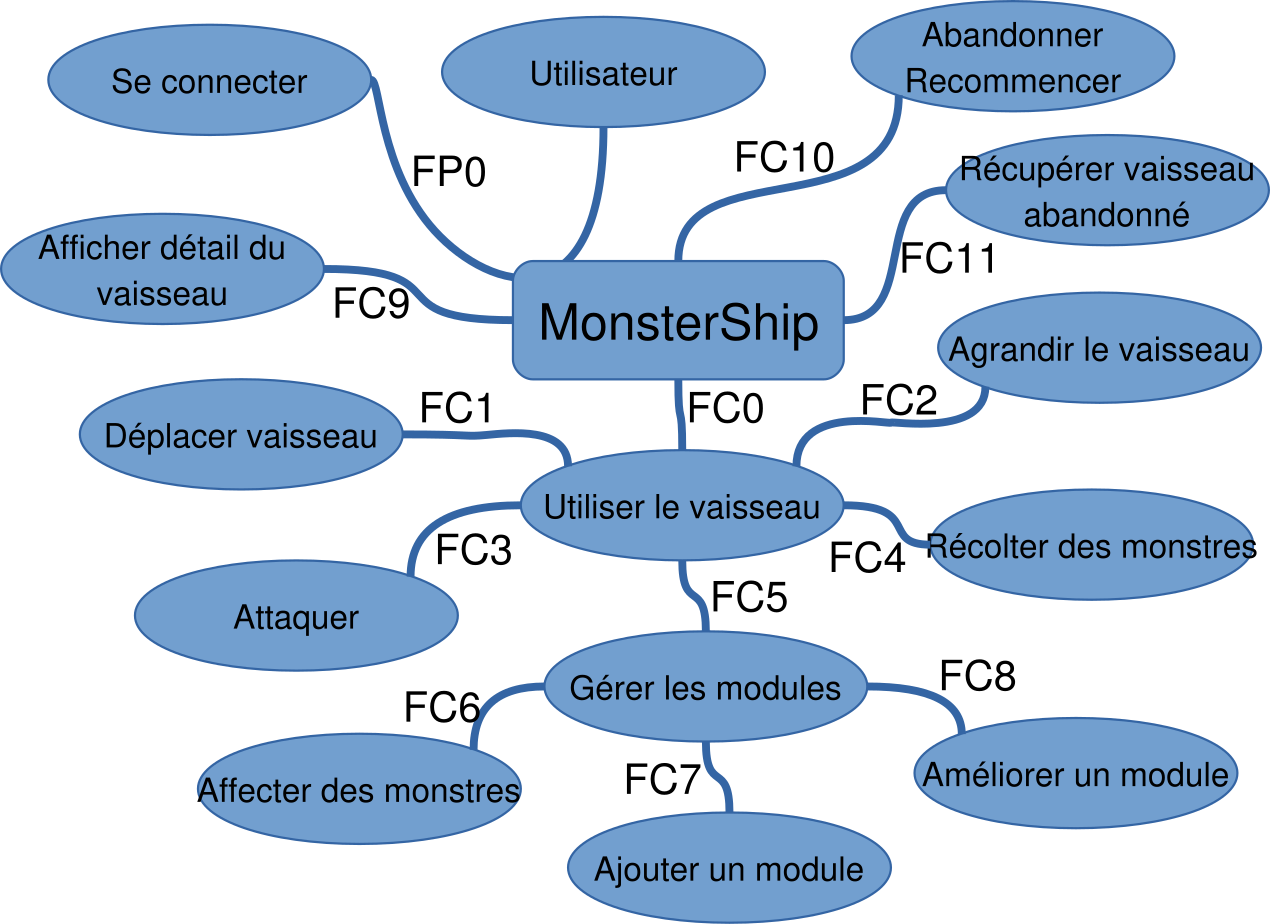
\includegraphics[width=\textwidth]{graphe_interactions/graphe_interactions.png}
                \caption{Graphe des intéractions}
                \label{fig:graphe_interactions}
            \end{center}
        \end{figure}

    \section{Les fonctions principales}
        \subsection{FP0 - Les utilisateurs se connectent à MonsterShip}
            Les utilisateurs accèdent à MonsterShip depuis leur navigateur internet. Une fois sur le site, ils peuvent se connecter pour commencer à jouer. L'accès au jeu est donc contrôlé, chaque utilisateur devant s'inscrire au préalable en fournissant un pseudonyme encore non utilisé.
    
    \section{Les fonctions complémentaires}
        \subsection{FC0 - Utiliser le vaisseau}
            Le jeu MonsterShip se concentre principalement sur la gestion de son vaisseau. À partir de cette fonction nous accédons donc à une grosse partie des fonctionnalités du jeu (FC1 à FC8).
        
        \subsection{FC1 - Déplacer son vaisseau}
            Pour explorer l'univers, l'utilisateur peut déplacer son vaisseau. Son vaisseau sera donc sur une grille où il pourra sélectionner une des cases à proximiter pour s'y déplacer. Selon la vitesse du vaisseau, il pourra sélectionner des cases plus lointaines. Un déplacement a un coup d'un point d'action.

        \subsection{FC2 - Agrandir le vaisseau}
            Dans l'objectif de faire prospérer son vaisseau. L'utilisateur peut être intéressé par le fait de faire agrandir son vaisseau. Il pourra ainsi accueillir plus de monstres.

        \subsection{FC3 - Attaquer}
            Une fois à distance d'attaque, l'utilisateur peut consommer un point d'action pour attaquer un vaisseau à proximiter. S'il est le vainqueur de la bataille, il récupérera des monstres du vaisseau adverse. S'il est le perdant, il repartira avec des dégâts, des modules peuvent être perdus en cas de défaite. Quand un joueur se fait attaquer, et qu'il gagne, il en ressort sans perte, ni gain. Cependant s'il est perdant, il est susceptible de perdre un ou plusieurs modules ainsi que des monstres.

        \subsection{FC4 - Récolter des monstres}
            À proximité d'une planète, le joueur peut y poser son vaisseau pour récolter des monstres. Deux possibilités s'offrent à lui :
            \begin{enumerate}
                \item Récolter immédiatement et retourner dans l'espace. Ce choix a l'avantage d'être immédiat et sans risque. Cependant il coûte un point d'action et le nombre de monstre qu'il peut récolter est plafonné.
                \item Récolter tant que le joueur ne décide pas de redécoller. Ce choix lui permet de récolter plus de monstres. Mais il doit pour cela se mettre en danger puisqu'il est susceptible de se faire attaquer dans une position désavantageuse. Cette méthode n'a aucun coût en point d'action.
            \end{enumerate}

        \subsection{FC5 - Gérer les modules}
            Cette fonctionnalité permet à l'utilisateur d'observer les améliorations possibles de modules, ainsi que l'ajout selon les ressources à sa disposition.

        \subsection{FC6 - Affecter des monstres}
            Pour qu'un module puisse fonctionner du mieux possible, il faut lui affecter des monstres.

        \subsection{FC7 - Ajouter un module}
            L'ajout de module coûte un certain nombre de monstre à fusionner, et il faut par la suite affecter des monstres à ce module pour qu'il puisse être fonctionnel. Tous les modules n'ont pas forcément le même coût.

        \subsection{FC8 - Améliorer un module}
            Il est possible d'améliorer des modules pour augmenter leurs statistiques. Les modules peuvent être améliorer pour différentes statistiques. Il est possible par exemple d'améliorer son propulseur de sorte qu'il soit plus performant pour les esquives en combat, ou bien améliorer sa vitesse pour explorer plus rapidement l'univers.

        \subsection{FC9 - Afficher détail du vaisseau}
            L'utilisateur a une vue d'ensemble de son vaisseau : le nombre de monstres à bord et les différentes statistiques du vaisseau.

        \subsection{FC10 - Abandonner recommencer}
            Un utilisateur peut à tout instant choisir d'abandonner son vaisseau pour recommencer avec un vaisseau de base ailleurs dans l'univers. Son vaisseau abandonné reste dans l'univers et pourra être découvert par un autre utilisateur ou par lui-même s'il le retrouve avant les autres joueurs. Au bout d'un certain temps (environ 1 semaine), le vaisseau disparaît.

        \subsection{FC11 - Récupérer vaisseau abandonné}
            Si un utilisateur tombe sur un vaisseau abandonné, il peut récupérer des monstres s'il en reste à bord.
    
\chapter{Maquette}
    \section{Page de connexion et d'inscription}
        \begin{figure}[H]
            \begin{center}
                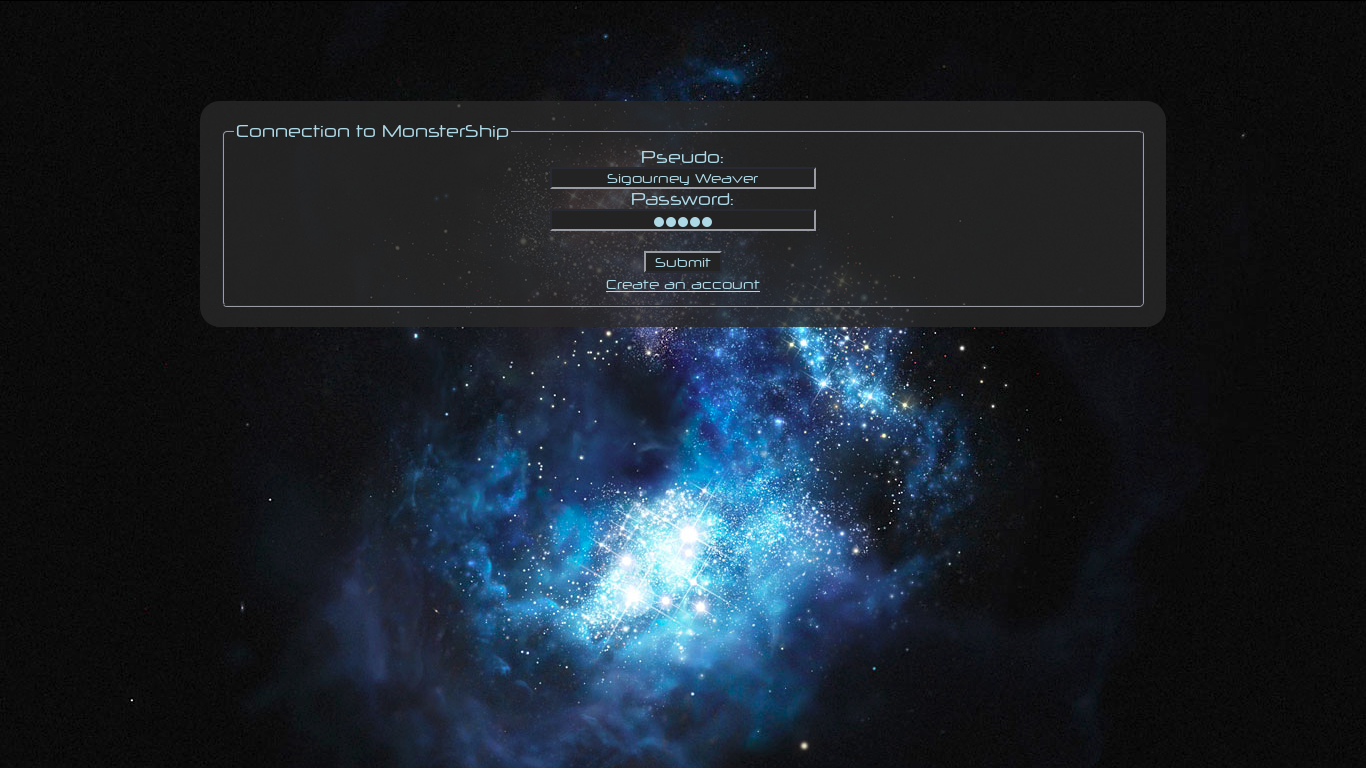
\includegraphics[width=\textwidth]{maquette/screens/login.png}
                \caption{Page de connexion}
                \label{fig:connexion}
            \end{center}
        \end{figure}
        \begin{figure}[H]
            \begin{center}
                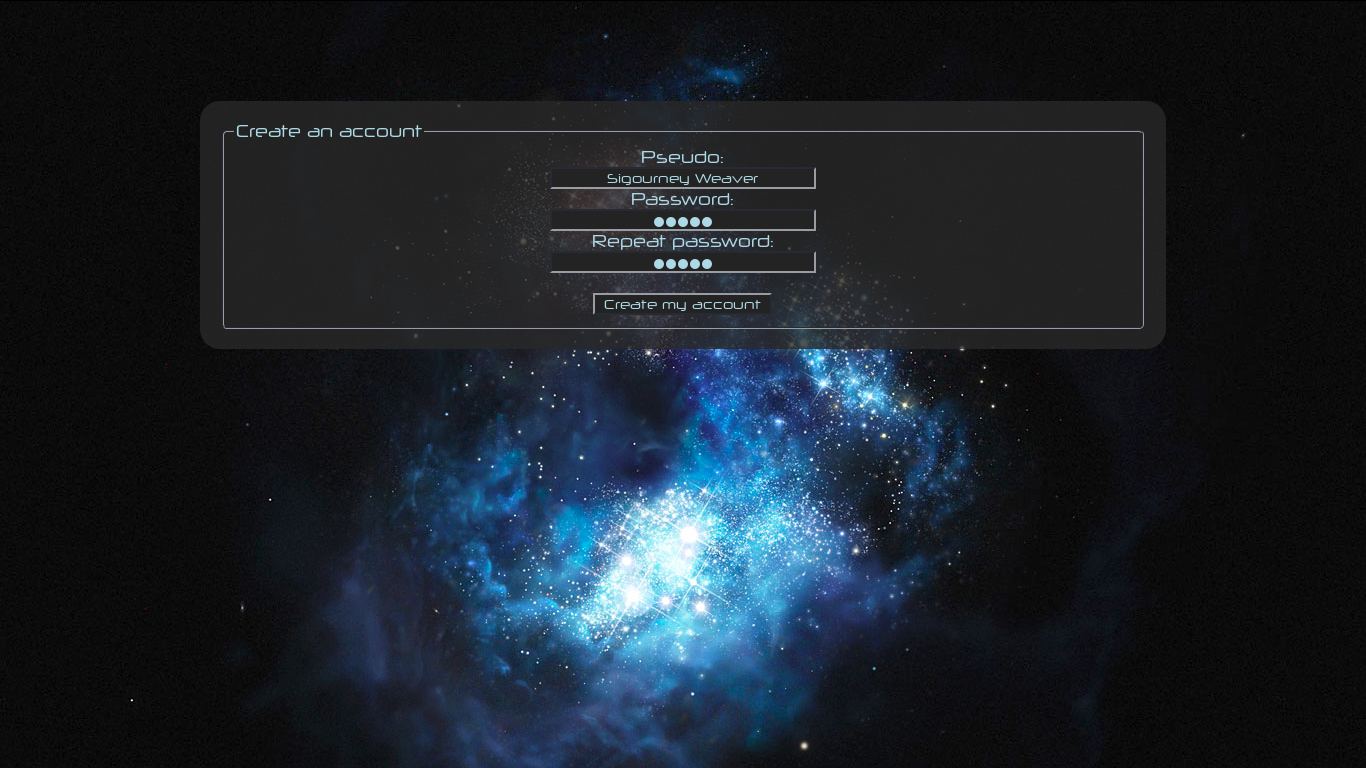
\includegraphics[width=\textwidth]{maquette/screens/registration.png}
                \caption{Page d'inscription}
                \label{fig:inscription}
            \end{center}
        \end{figure}
        Pour l'inscription, il n'est demandé qu'un nom d'utilisateur et un mot de passe (qu'il faut répéter pour être sûr que l'utilisateur ne se trompe pas). Plus d'informations seraient superflus.

    \section{Page principale}
        \begin{figure}[H]
            \begin{center}
                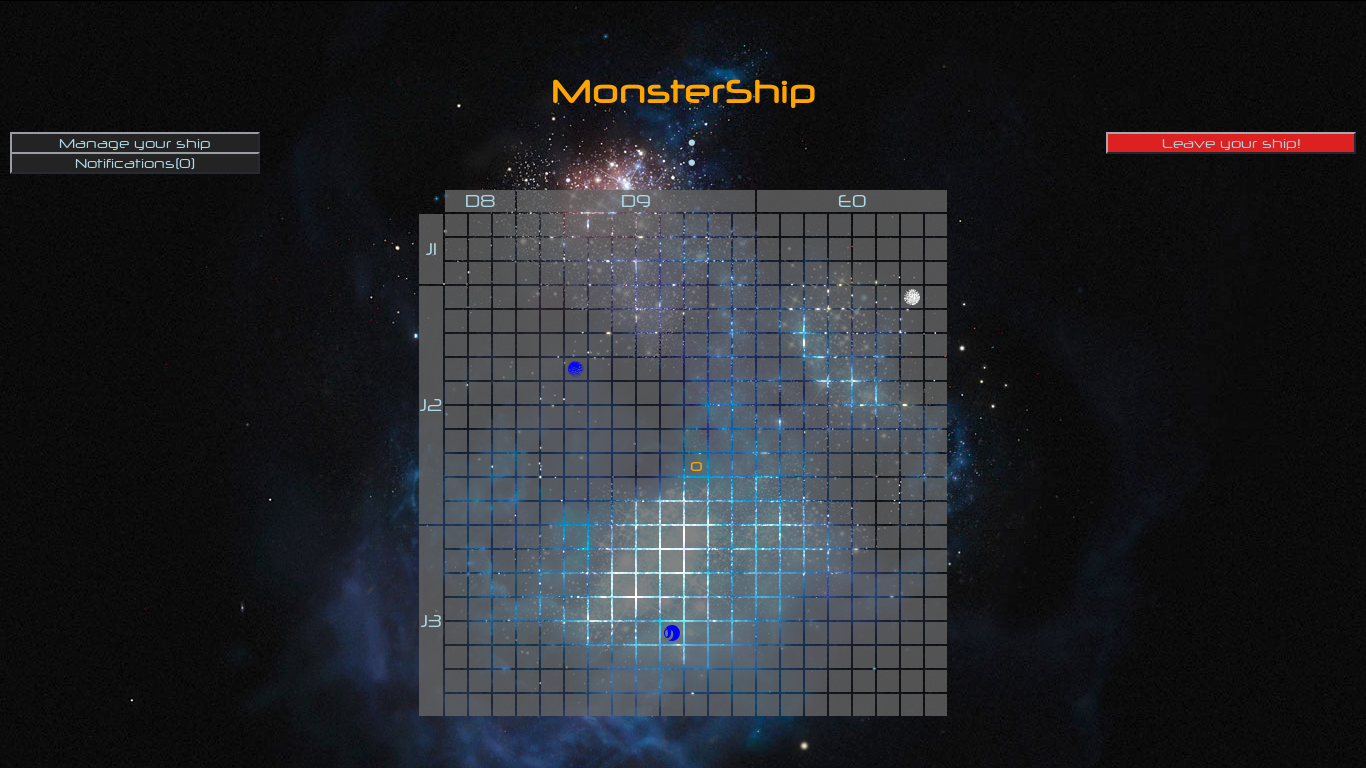
\includegraphics[width=\textwidth]{maquette/screens/main.png}
                \caption{Page principale du jeu}
                \label{fig:principale}
            \end{center}
        \end{figure}
        Le vaisseau est au centre de la map. Nous voyons 3 planètes sur la carte. Nous avons un bouton pour accéder à l'interface de gestion du vaisseau (pour ajouter des modules, gérer notre équipage), un autre pour les notifications (rapport de combat quand on se fait attaquer par exemple) et un bouton à droite pour l'abandon du vaisseau.\\

        En dessous des notifications, il sera possible de placer les boutons d'actions, si par exemple on est à proximité d'un autre vaisseau.

    \section{Page de gestion du vaisseau}
        \begin{figure}[H]
            \begin{center}
                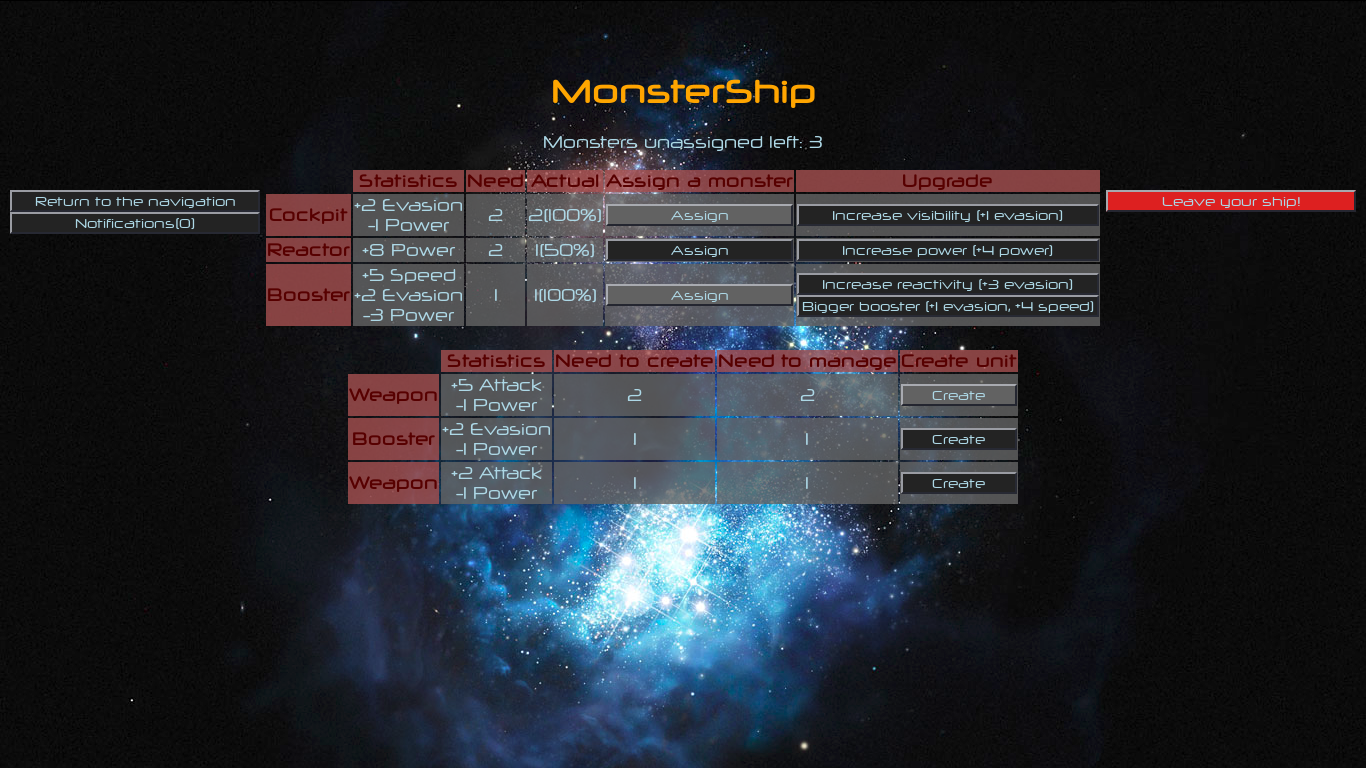
\includegraphics[width=\textwidth]{maquette/screens/manage.png}
                \caption{Page de gestion du vaisseau}
                \label{fig:gestion}
            \end{center}
        \end{figure}
        Nous avons deux tableaux, le premier permet de voir les modules composant notre vaisseau, leurs statistiques, le nombre de monstre nécessaire pour leur bon fonctionnement et les améliorations possibles. Le second tableau permet d'ajouter des modules à ceux existants.

\chapter{Organisation et gestion du temps}
    \section{Visualisation du projet dans le temps}
        \begin{figure}[H]
            \begin{center}
                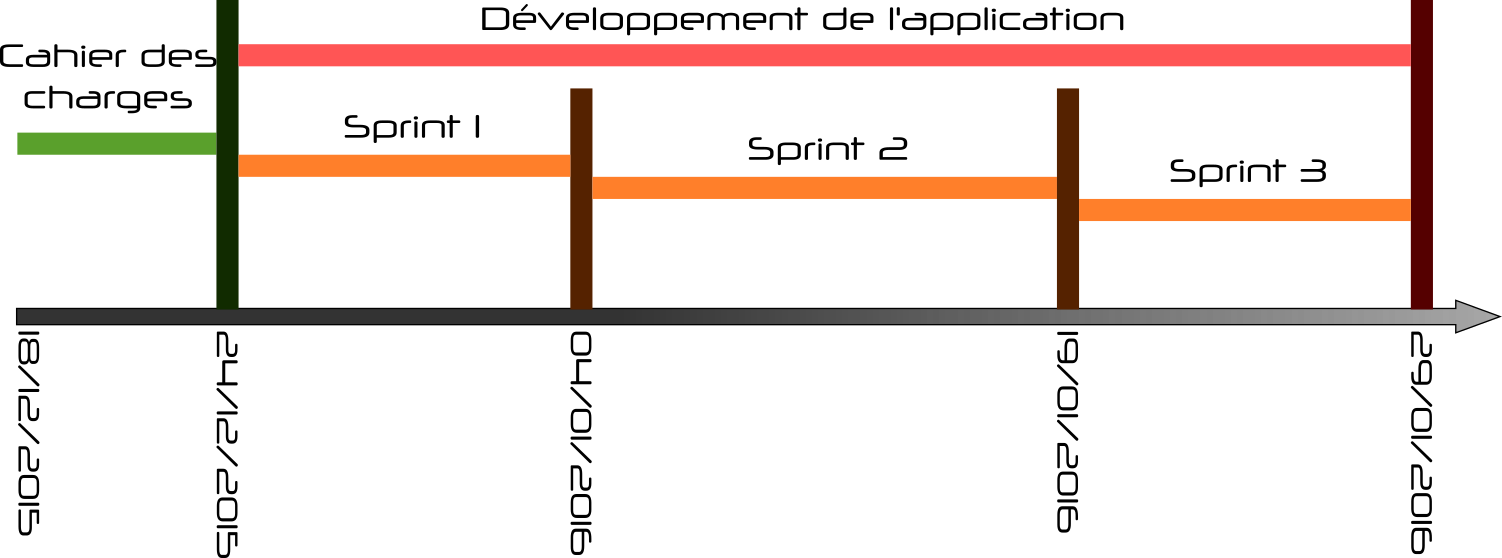
\includegraphics[width=\textwidth]{gantt/gantt.png}
                \caption{Harmonogram Adamieckiego}
                \label{fig:gantt}
            \end{center}
        \end{figure}
        Les sprints n'ont pas rigoureusement le même temps pour que les dates correspondant aux bilans des sprints coïncident avec des journées où l'équipe peut se rencontrer.
        \begin{description}
            \item[Sprint 1] Mise en place de la structure du projet (côté serveur, mais aussi côté client). Développement des premières fonctionnalités : inscription, connexion, déplacement du vaisseau dans l'espace et la possibilité d'abandonner son vaisseau.
            \item[Sprint 2] Développement des parties : gestion des modules, récolte de monstres (sur des planètes ou des vaisseaux abandonnés) et la possibilité de s'attaquer entre joueurs.
            \item[Sprint 3] Développement des parties : agrandissement du vaisseau, ajout de contenu (modules, améliorations), équilibrage des stastiques des modules et des mécanismes de jeu.
        \end{description}

    \section{Structure du projet} 
        \begin{figure}[H]
            \begin{center}
                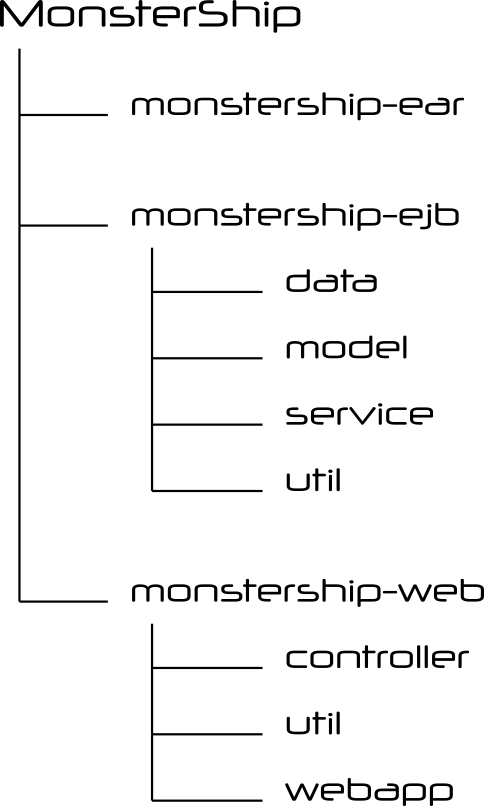
\includegraphics[width=.5\textwidth]{structure_projet/structure_projet.png}
                \caption{Arborescence du projet}
                \label{fig:arbo}
            \end{center}
        \end{figure}
        \begin{description}
            \item[monstership-ear] cette partie permet d'empacter les modules du projet
            \item[monstership-ejb] nous développerons les entités dans cette partie
            \begin{description}
                \item[data] définit l'accès aux données
                \item[model] définit la structure de données du projet
                \item[service] gère les fonctionnalités de l'application (inscription, connexion, déplacement du vaisseau, etc)
                \item[util] c'est la partie outillage, on peut y mettre un système de log par exemple 
            \end{description}
            \item[monstership-web] est l'application web qu'utiliseront les joueurs
            \begin{description}
                \item[controller] définit comment gérer les événements
                \item[util] de même que l'ejb
                \item[webapp] c'est la vue de l'application 
            \end{description}
        \end{description}
        \begin{figure}[H]
            \begin{center}
                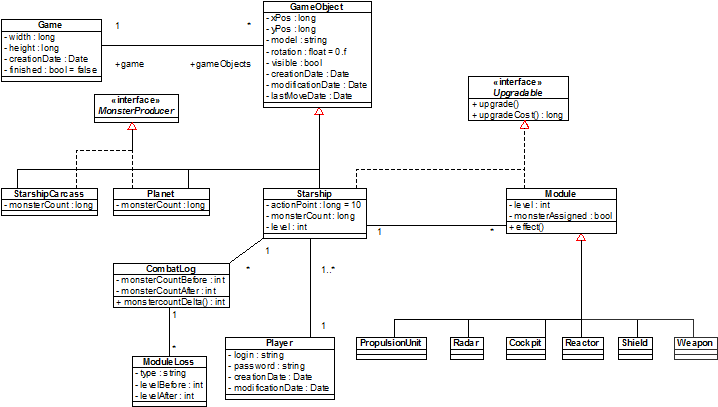
\includegraphics[width=\textwidth]{cls_diag/class_diagram.png}
                \caption{Diagramme de classe}
                \label{fig:classe}
            \end{center}
        \end{figure}

\end{document}
